\documentclass[11pt,a4paper]{article}

\usepackage[margin=2.4cm]{geometry}
\usepackage{amsmath}
\usepackage{fontspec}
\usepackage{tikz}
\usepackage{booktabs}
\usepackage{array}
\usepackage{xcolor}
\usepackage{titlesec}
\usepackage{enumitem}
\usepackage{caption}
\usepackage[hidelinks]{hyperref}
\usetikzlibrary{arrows.meta, positioning, fit, backgrounds, calc}

% ---------------------------------------------------------------- fonts ----
\setmainfont{Palatino}
\newfontfamily\bn{Kohinoor Bangla}[Script=Bengali]
\newcommand{\bng}[1]{{\bn #1}}

% --------------------------------------------------------------- colours ---
\definecolor{ink}{HTML}{14161F}
\definecolor{muted}{HTML}{6B7280}
\definecolor{accent}{HTML}{4F46E5}
\definecolor{confident}{HTML}{0E9F6E}
\definecolor{uncertain}{HTML}{D97706}
\definecolor{rule}{HTML}{D8D5CC}
\definecolor{paper}{HTML}{F7F6F2}

\titleformat{\section}{\large\bfseries\color{ink}}{\thesection}{0.7em}{}
\titleformat{\subsection}{\normalsize\bfseries\color{ink}}{\thesubsection}{0.6em}{}
\titlespacing*{\section}{0pt}{1.5em}{0.6em}
\titlespacing*{\subsection}{0pt}{1.1em}{0.4em}

\captionsetup{font={small,color=muted}, labelfont={bf,color=accent}}

\setlist[itemize]{leftmargin=1.3em, itemsep=2pt, topsep=3pt}
\newcommand{\code}[1]{\texttt{\small #1}}

\begin{document}

% ============================================================== title ======
\begin{titlepage}
\centering
\vspace*{3.2cm}

{\Huge\bfseries\color{ink} Muse\par}
\vspace{0.4cm}
{\LARGE\color{accent} Structured Field Intelligence from\\[2mm] Noisy Bangla Speech and Handwriting\par}

\vspace{1.0cm}
{\large\bng{মিউজ}\par}

\vspace{2.0cm}
\begin{minipage}{0.82\textwidth}
\centering\itshape\color{muted}
A voice- and image-driven capture pipeline that recovers reliable structured
data from Bangla field reports at word error rates near 34\%, using a
deterministic linguistic layer and constrained generation rather than a larger
acoustic model.
\end{minipage}

\vfill
{\color{muted}\small BrainChild 2.0 \quad$\cdot$\quad Jagannath University AI \& IT Fest\par}
{\color{muted}\small August 2026\par}
\end{titlepage}

% =========================================================== abstract ======
\section*{Abstract}
\noindent
Bangladesh's FMCG sector is a roughly USD~4 billion market in which about 97\%
of trade flows through traditional retail: small, independent shops visited in
person by distribution representatives. Sales-force automation captures the
transaction from those visits but not the observation---why a shop refused an
order, what a competitor is running, what a retailer complained about. That
information is never recorded, because typing several sentences at forty
outlets a day is not feasible.

Muse captures it by voice and by photograph of the handwritten order note. The
central difficulty is that Bangla speech recognition, which reports 3--5\% word
error rate on clean read benchmarks, degrades to approximately 34\% on real
long-form field audio. Rather than pursue a better acoustic model, Muse treats
the transcript as unreliable by design and recovers the \emph{fields} through a
deterministic layer: a Bangla quantity grammar covering the fractional and
multiplicative forms that general models mishandle, and phonetic normalisation
that folds Bangla orthography and Latin catalogue names into a shared key
space. A language model is then constrained per recording to a vocabulary the
resolvers actually produced, making an unresolvable product inexpressible
rather than merely discouraged. Confidence is derived from upstream evidence,
never self-reported, and gates a one-tap clarification returned to the
representative. The system comprises 412 automated tests; the deterministic
layer accounts for roughly 40\,ms of a 2.4\,s pipeline.

% ======================================================== introduction =====
\section{Problem}

A distribution representative in Dhaka observes a competitor promotion running
across twelve shops on a Tuesday. Under current practice his brand manager
learns of it weeks later, inferred from a sales decline. The delay is not a
failure of diligence; it is structural. Sales-force automation systems record
order quantity, SKU, outlet and timestamp. They provide no mechanism for the
unstructured observation, and no realistic mechanism could: the representative
has fifteen seconds per shop and both hands occupied.

The consequence is measurable. Published estimates place the global average
retail out-of-stock rate at approximately 8.3\%, and find that 58\% of shoppers
encountering a stock-out do not defer the purchase but abandon it. Shortening
the interval between a field observation and a decision is therefore a revenue
protection problem, not a labour cost problem---a distinction that matters in a
market where a representative's monthly wage does not justify automation on
cost grounds alone.

\subsection{Why existing approaches do not address it}

\begin{table}[h]
\centering\small
\begin{tabular}{@{}p{3.4cm} p{4.6cm} p{6.2cm}@{}}
\toprule
\textbf{Approach} & \textbf{Captures} & \textbf{Does not capture} \\
\midrule
Sales-force automation & Orders, GPS check-in, route compliance & Any unstructured observation \\
Retail audit panels & Rigorous, comparable measurement & Sample-based and monthly; reports the previous period \\
Messaging groups & Ad-hoc photographs and text & Unstructured, unsearchable, not aggregable \\
Additional headcount & More visits & The same capture limitation, multiplied \\
General speech-to-text & A transcript & Product resolution, confidence, Bangla numerals \\
\bottomrule
\end{tabular}
\caption{A transcript is not data. The gap is between recognised text and a resolved, checkable field.}
\end{table}

% ======================================================== architecture =====
\section{System architecture}

Muse is a six-stage pipeline. Two stages call external models; the remaining
four are domain logic. Both capture modalities---voice and photograph---diverge
for exactly one stage and share everything after it.

\begin{figure}[h]
\centering
\resizebox{\textwidth}{!}{%
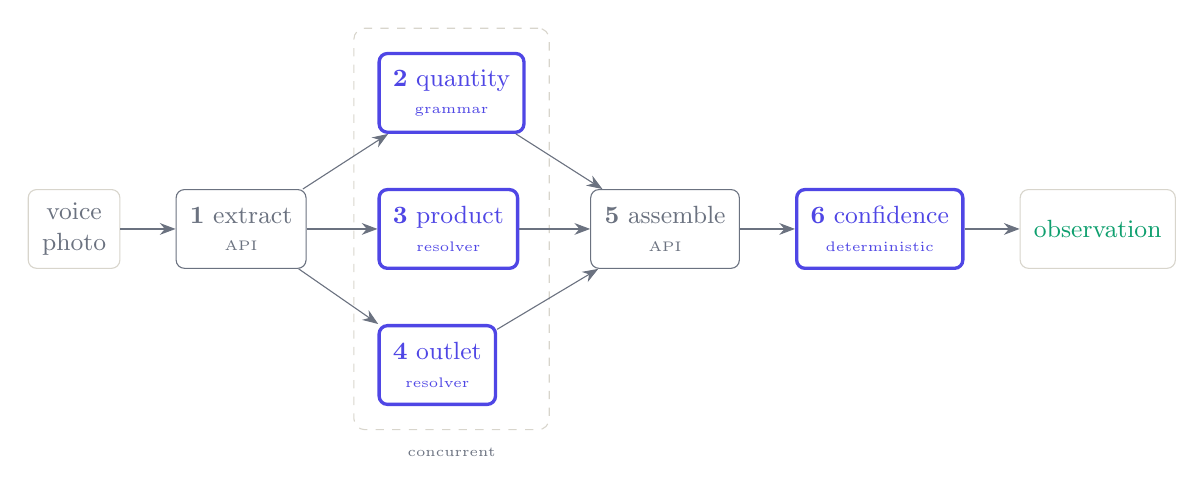
\begin{tikzpicture}[
  font=\small,
  box/.style={draw=rule, fill=white, rounded corners=3pt, minimum height=10mm,
              inner xsep=5pt, align=center},
  api/.style={box, draw=muted, text=muted},
  own/.style={box, draw=accent, very thick, text=accent},
  ar/.style={-{Stealth[length=2mm]}, draw=muted}
]
\node[box, text=muted] (in) {voice\\photo};
\node[api, right=7mm of in] (ex) {\textbf{1} extract\\[-1pt]{\tiny API}};
\node[own, above right=7mm and 9mm of ex] (q) {\textbf{2} quantity\\[-1pt]{\tiny grammar}};
\node[own, right=9mm of ex] (s) {\textbf{3} product\\[-1pt]{\tiny resolver}};
\node[own, below right=7mm and 9mm of ex] (o) {\textbf{4} outlet\\[-1pt]{\tiny resolver}};
\node[api, right=9mm of s] (as) {\textbf{5} assemble\\[-1pt]{\tiny API}};
\node[own, right=7mm of as] (c) {\textbf{6} confidence\\[-1pt]{\tiny deterministic}};
\node[box, text=confident, right=7mm of c] (out) {observation};

\draw[ar] (in) -- (ex);
\draw[ar] (ex) -- (q); \draw[ar] (ex) -- (s); \draw[ar] (ex) -- (o);
\draw[ar] (q) -- (as); \draw[ar] (s) -- (as); \draw[ar] (o) -- (as);
\draw[ar] (as) -- (c);
\draw[ar] (c) -- (out);

\begin{scope}[on background layer]
\node[fit=(q)(o), draw=rule, dashed, rounded corners, inner sep=3mm] (par) {};
\end{scope}
\node[below=1mm of par, text=muted, font=\tiny] {concurrent};
\end{tikzpicture}}
\caption{Stages 2--4 are independent and run concurrently; they annotate a shared transcript without modifying it. Blue stages are domain logic; grey stages are external model calls.}
\end{figure}

Two invariants hold throughout. First, stages annotate but never rewrite the
transcript: each annotation carries character offsets into the original text,
so a later stage can inspect the evidence that produced a value. Second, the
extraction stage is the only point at which voice and photograph differ, which
is what allowed a second modality to be added by modifying four files.

% ==================================================== contributions ========
\section{Technical approach}

\subsection{A Bangla quantity grammar}

Bangla expresses quantity with fractional prefixes and multiplicative units
that general-purpose models handle unreliably. The grammar resolves these
deterministically.

\begin{table}[h]
\centering\small
\begin{tabular}{@{}l l l | l l l@{}}
\toprule
\multicolumn{3}{c|}{\textbf{Fractional}} & \multicolumn{3}{c}{\textbf{Multiplicative}}\\
Form & Value & & Form & Value & \\
\midrule
\bng{দেড়}   & $1.5$        & standalone & \bng{ডজন}  & $\times 12$ & dozen \\
\bng{আড়াই}  & $2.5$        & standalone & \bng{হালি}  & $\times 4$  & set of four \\
\bng{সাড়ে} X & $X + 0.5$    & prefix     & \bng{কুড়ি}  & $\times 20$ & score \\
\bng{সোয়া} X & $X + 0.25$   & prefix     & \bng{গণ্ডা} & $\times 4$  & \\
\bng{পৌনে} X & $X - 0.25$   & \textbf{subtracts} & \bng{লাখ} & $\times 10^5$ & \\
\bottomrule
\end{tabular}
\caption{\bng{পৌনে} subtracts, which naive keyword matching inverts. \bng{দেড় ডজন} evaluates to $1.5 \times 12 = 18$ pieces.}
\end{table}

\subsection{Phonetic normalisation}

Bangla orthography maps many graphemes onto one sound, and speech recognition
loses these distinctions first. Both the recognised text and the product
catalogue are folded into a shared phonetic key space, which also absorbs the
script boundary: catalogues are written in English while representatives speak
Bangla.

\begin{table}[h]
\centering\small
\begin{tabular}{@{}l l | l l@{}}
\toprule
\textbf{Collapse} & \textbf{Key} & \textbf{Heard} & \textbf{Resolves to} \\
\midrule
\bng{শ}\,\bng{ষ}\,\bng{স} & \code{s} & \bng{হইল} $\rightarrow$ \code{huil} & Wheel $\rightarrow$ \code{huil} \\
\bng{ণ}\,\bng{ন} & \code{n} & \bng{প্রান} $\rightarrow$ \code{pran} & PRAN $\rightarrow$ \code{pran} \\
\bng{র}\,\bng{ড়}\,\bng{ঢ়} & \code{r} & \bng{ম্যাঙ্গো} $\rightarrow$ \code{mango} & Mango $\rightarrow$ \code{mango} \\
vowel length, aspiration & --- & \bng{তীন} $\rightarrow$ \code{tin} & \bng{তিন} $\rightarrow$ \code{tin} \\
\bottomrule
\end{tabular}
\caption{Word-initial Latin ``wh'' maps to \code{hu}, since Bengali renders it \bng{হু}. Without this the brand never matches its own catalogue entry.}
\end{table}

Two comparison modes are required. Product and outlet names use a lenient
comparison that also considers the consonant skeleton, since vowels are the
least reliable signal. The numeral lexicon uses a strict comparison retaining
vowels: \bng{সতেরো} (seventeen) and \bng{স্টোরে} (``at the store'') share the
skeleton \code{s-t-r} exactly, and a lenient comparison reads a shop as a
number.

\subsection{Constrained generation}

A language model performs segmentation and semantics only. Its response schema
is rebuilt for every recording, with identity fields restricted to an
enumeration of exactly the candidates the resolvers produced:

\begin{center}\small
\code{skuId: enum(["SKU-404", "SKU-407"]).nullable()}
\end{center}

A product that was not resolved is therefore not expressible. This is a
structural constraint rather than an instruction, and it is what makes the
system deployable where a confidently incorrect SKU is worse than no record.
Numeric fields receive a second guard, since a schema cannot bind a float:
any quantity the model returns is checked against what the grammar parsed and
discarded otherwise.

\subsection{Derived confidence and clarification}

Confidence is computed from upstream evidence and never requested from the
model, which is poorly calibrated and will assign high confidence to invented
values.

\[
  \text{conf}(f) \;=\; \text{asr}(\text{span}_f) \;\times\; m(\text{margin}) \;\times\; g(\text{grammar})
\]

The margin term---the gap between the resolver's first and second
candidate---is decisive. A high top score with a narrow margin indicates that
two products are indistinguishable, and gating on score alone would confirm
precisely those cases.

\begin{figure}[h]
\centering
\resizebox{0.96\textwidth}{!}{%
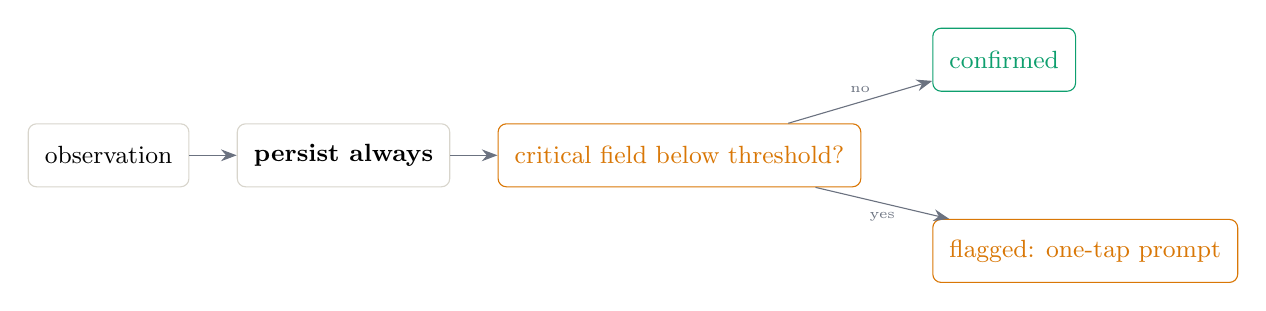
\begin{tikzpicture}[
  font=\small, node distance=6mm,
  b/.style={draw=rule, fill=white, rounded corners=3pt, minimum height=8mm, inner xsep=6pt},
  d/.style={draw=uncertain, fill=white, rounded corners=3pt, minimum height=8mm, inner xsep=6pt, text=uncertain},
  ar/.style={-{Stealth[length=2mm]}, draw=muted}
]
\node[b] (o) {observation};
\node[b, right=of o] (save) {\textbf{persist always}};
\node[d, right=of save] (q) {critical field below threshold?};
\node[b, above right=4mm and 9mm of q, text=confident, draw=confident] (ok) {confirmed};
\node[d, below right=4mm and 9mm of q] (fl) {flagged: one-tap prompt};
\draw[ar] (o) -- (save);
\draw[ar] (save) -- (q);
\draw[ar] (q) -- node[above, font=\tiny, text=muted] {no} (ok);
\draw[ar] (q) -- node[below, font=\tiny, text=muted] {yes} (fl);
\end{tikzpicture}}
\caption{Low confidence sets a status; it never discards a record. A dropped observation is unusable in an enterprise, whereas a flagged one is merely honest.}
\end{figure}

An unanswered prompt resolves to the best guess after a fixed interval, and an
answer arriving after that resolution still applies---the record was already
published with a guess, so a late correction must reach the dashboard.

% ======================================================== results ==========
\section{Implementation and results}

The system is implemented in TypeScript across an Express API, a queue worker
and a React client, with MongoDB and Redis. Pipeline stages are dependency-free
classes constructed with ports, so the test suite requires no container.

\subsection{Worked example}

The following is verbatim output from a production speech model on real audio.

\begin{center}\small
\begin{tabular}{@{}p{0.93\textwidth}@{}}
\toprule
\textbf{Recognised:} \bng{বজোই স্তোর মে প্রান মাঙ্গো জুস দের দর্জন লগেগা} \\
\midrule
\textbf{Recovered:} Bijoy Store (0.79) $\cdot$ PRAN Mango Juice 250ml (0.98) $\cdot$ 18 piece (0.85)\\
\bottomrule
\end{tabular}
\end{center}

Four words are mis-transcribed---the outlet name, the brand, and the numeral
phrase---and every field is nonetheless correct. This is the intended
behaviour rather than a fortunate case: the resolvers never consult the
transcript for correctness, only for similarity against a closed catalogue.

\subsection{Measured characteristics}

\begin{table}[h]
\centering\small
\begin{tabular}{@{}l r l@{}}
\toprule
\textbf{Measure} & \textbf{Value} & \textbf{Note} \\
\midrule
Automated tests & 412 & full suite under 1\,s, no network \\
Deterministic layer latency & $\approx$40\,ms & of a $\approx$2.4\,s pipeline \\
Extraction latency & 450--1250\,ms & external model call \\
Assembly latency & $\approx$1.9\,s & external model call \\
Files changed to add photograph capture & 4 & \\
\bottomrule
\end{tabular}
\caption{Nearly all latency is external model calls; the domain logic is negligible by comparison.}
\end{table}

% ======================================================= business =========
\section{Economic model}

The following is a model, not a measurement, and is presented with its
assumptions stated. For a brand covering 10{,}000 outlets at BDT~25{,}000
monthly sell-through each (BDT~3.0\,billion annually):

\begin{table}[h]
\centering\small
\begin{tabular}{@{}l r l@{}}
\toprule
Out-of-stock rate & 8.3\% & published \\
Share becoming lost sales & 58\% & published \\
Revenue lost to stock-outs & 4.8\% & derived \\
& BDT~144\,M & per year \\
\midrule
Reduction from same-day reporting & 20\% & \textbf{assumed} \\
Recovered & BDT~28.8\,M & per year \\
Platform cost (150 representatives) & BDT~2.16\,M & per year \\
\midrule
\textbf{Return} & $\approx$\textbf{13$\times$} & \\
\bottomrule
\end{tabular}
\caption{Only the 20\% reduction is assumed; halving it still yields roughly a sixfold return.}
\end{table}

% ==================================================== limitations =========
\section{Limitations and further work}

\begin{itemize}
  \item \textbf{Dialect.} Version one targets Dhaka-standard Bangla. Chittagonian
        and Sylheti are effectively distinct languages for a speech model and
        are explicitly out of scope.
  \item \textbf{Handwriting recognition is simulated} in the current build. Text
        extracted from a photograph is canned; every stage after extraction is
        the production pipeline, and this is disclosed in the interface itself.
  \item \textbf{Evaluation.} A harness measuring word error rate, per-field
        precision and confidence calibration is implemented and gated on
        regression, but requires a labelled corpus of field recordings that has
        not yet been collected. No accuracy figure is claimed here for that reason.
  \item \textbf{Unmatched surface forms} produce no annotation and therefore cannot
        enter the alias-learning queue---precisely the case where an alias would
        help most. Addressing this requires the resolver to emit sub-threshold
        near-misses.
\end{itemize}

Planned work includes domain-adapted Bangla speech recognition through n-gram
shallow fusion over the customer catalogue, a learned confidence model trained
on the evaluation corpus, and genuine optical character recognition for printed
signage. The architecture generalises to other Bangla-speaking field forces---%
pharmaceutical representatives, microfinance officers, agricultural extension
workers---by substituting the catalogue and observation schema.

% ==================================================== references =========
\section*{References}
\small
\begin{enumerate}[leftmargin=1.6em, itemsep=1pt]
  \item The Business Standard / FICCI. Bangladesh FMCG market size and composition.
  \item IHL Group. \emph{Retail Inventory Crisis Persists Despite \$172 Billion in Improvements}, 2025.
  \item Zebra Technologies. \emph{Global Shopper Study}---stock-out conversion to lost sales.
  \item FLEURS and Common Voice Bengali benchmarks; published long-form Bangla ASR evaluations.
\end{enumerate}

\end{document}
